\documentclass[a4paper, 11pt]{report}

% --- Encodage et Langue ---
\usepackage[T1]{fontenc}
\usepackage[utf8]{inputenc}
\usepackage[french]{babel}

% --- Polices et Mise en page ---
\usepackage{helvet}
\renewcommand{\familydefault}{\sfdefault}
\usepackage{setspace}
\setstretch{1.15}
\usepackage{geometry}
\geometry{hmargin=2.5cm, vmargin=3cm}

% --- Mathématiques et Graphiques ---
\usepackage{amsmath}
\usepackage{graphicx}
\graphicspath{{images/}}

% --- Listings de code (PDDL, Python, Bash) ---
\usepackage{xcolor}
\usepackage{listings}

\definecolor{codebg}{RGB}{248,248,248}
\definecolor{codecomment}{RGB}{110,110,110}
\definecolor{codekeyword}{RGB}{0,90,160}
\definecolor{codestring}{RGB}{160,60,30}

\lstdefinestyle{base}{
	backgroundcolor=\color{codebg},
	basicstyle=\ttfamily\small,
	commentstyle=\color{codecomment}\itshape,
	keywordstyle=\color{codekeyword}\bfseries,
	stringstyle=\color{codestring},
	numbers=left,
	numberstyle=\tiny\color{codecomment},
	numbersep=8pt,
	frame=single,
	rulecolor=\color{codecomment},
	breaklines=true,
	showstringspaces=false,
	tabsize=2,
	captionpos=b
}

\lstdefinelanguage{pddl}{
	morekeywords={define,domain,problem,requirements,types,predicates,action,
		parameters,precondition,effect,objects,init,goal,and,not,
		robot,room,strips,typing},
	sensitive=true,
	morecomment=[l]{;}
}

\lstdefinelanguage{bash}{
	morekeywords={sudo,apt,update,install,cd,git,clone,python3,ls,mkdir,cp,mv,rm,echo,export,source,cat},
	sensitive=true,
	morecomment=[l]{\#}
}

\lstdefinestyle{pddl}{style=base,language=pddl}
\lstdefinestyle{python}{style=base,language=Python}
\lstdefinestyle{bash}{style=base,language=bash}

\lstset{style=base}

% --- Tableaux ---
\usepackage{array}

% --- Utilitaires et Liens ---
\usepackage[pdfpagelabels=false]{hyperref}

% --- Annexes ---
\renewcommand{\appendixname}{Annexe}
\renewcommand{\appendixtocname}{Annexes}
\renewcommand{\appendixpagename}{Annexes}

\begin{document}
	
	% ============================================================
	% PAGE DE GARDE
	% ============================================================
	\begin{titlepage}
		\centering
		{\Huge\bfseries UNIVERSITÉ DE KINSHASA\par}
		\vspace{0.2cm}
		
		
\includegraphics[width=0.12\textwidth]{images/image.png}\\
		\vspace{0.3cm}
		\textsc{\large \textbf{FACULTÉ DES SCIENCES ET TECHNOLOGIES \\
				Mention : INFORMATIQUE}}\\
		\href{mailto:departement.mathinfo@unikin.ac.cd}
		{\texttt{departement.mathinfo@unikin.ac.cd}}\\
		\underline{B.P. 190 KINSHASA XI}\\
		\vfill
		
		\rule{\textwidth}{2pt}\\[0.3cm]
		{\huge Planification en Intelligence Artificielle\\[0.3cm]
			\Large\bfseries Sujet 2 : Robot Aspirateur en PDDL et Fast Downward\\[0.3cm]}
		\rule{\textwidth}{2pt}\\
		\vfill
		
		{\small\bfseries Réalisé par\par}
		\begin{center}
			\large
			\renewcommand{\arraystretch}{1.5}
			\begin{tabular}{l c c l c}
				1. KIMBUNGU SIMEON Gédéon     & [\quad] & \hspace{0.5cm} & 4. TANDU KIKALANGA Nathan   & [\quad] \\
				2. LABEM KAPINGA Ketsia       & [\quad] & \hspace{0.5cm} & 5. LUNGA KABITA Supreme     & [\quad] \\
				3. KALEMBU MASIRIKA Constantin & [\quad] & \hspace{0.5cm} &                             &          \\
			\end{tabular}
		\end{center}
		
		\vspace{0.4cm}
		{\large Promotion Master 1 / Informatique}\\
		\vspace{0.8cm}
		
		\begin{flushleft}
			\vspace{0.5cm}
			\begin{tabular}{ll}
				Domaine    & : Sciences et Technologies \\
				Professeur & : \textbf{Doctorant. Patrick MANYA} \\
			\end{tabular}
		\end{flushleft}
		
		\vfill
		{\large Année Académique 2025--2026\par}
	\end{titlepage}
	
	% ============================================================
	% TABLE DES MATIÈRES
	% ============================================================
	\tableofcontents
	\newpage
	
	% ============================================================
	% CORPS DU RAPPORT
	% ============================================================
	
	\section{Introduction}
	
	Ce travail s'inscrit dans le cadre du cours de planification en intelligence
	artificielle. Il nous demandait de choisir un problème de planification
	classique, de le modéliser en STRIPS/PDDL, puis de le soumettre à un
	planificateur automatique afin d'obtenir un plan d'actions. Nous avons choisi
	le sujet du robot aspirateur dans un logement composé de plusieurs pièces.
	
	Le problème que nous nous sommes posé est le suivant : un robot doit nettoyer
	toutes les pièces d'un logement, mais il ne peut se déplacer qu'entre pièces
	reliées par un passage. Il ne peut pas nettoyer une pièce sans y être, et il
	ne peut pas se téléporter d'une pièce à une autre. Il faut donc trouver un
	ordre de visite et de nettoyage qui permette d'atteindre l'objectif, en
	respectant à chaque étape les contraintes du logement.
	
	Pour répondre à cette question, nous avons d'abord modélisé le logement et le
	comportement du robot en PDDL. Nous avons ensuite utilisé le planificateur
	Fast Downward pour générer un plan. Enfin, nous avons écrit un simulateur en
	Python pour rejouer ce plan et vérifier qu'il était effectivement exécutable.
	Le rapport suit ce déroulement : il présente la modélisation, le domaine et
	le problème PDDL, l'exécution avec Fast Downward, la vérification en Python,
	puis deux scénarios alternatifs qui montrent comment le plan s'adapte lorsque
	l'on modifie l'état initial ou la topologie du logement.
	
	\section{Modélisation du problème}
	
	\subsection{Description du logement}
	
	Le logement que nous avons choisi comporte quatre pièces : la cuisine, le
	salon, la chambre et la salle de bain. Ces pièces ne communiquent pas toutes
	entre elles. Le salon joue le rôle de nœud central : il est relié
	directement à la cuisine, à la chambre et à la salle de bain, alors
	qu'aucune de ces trois pièces n'est reliée directement aux deux autres. Pour
	aller de la cuisine à la chambre, par exemple, le robot doit obligatoirement
	traverser le salon.
	
	\begin{figure}[h]
		\centering
		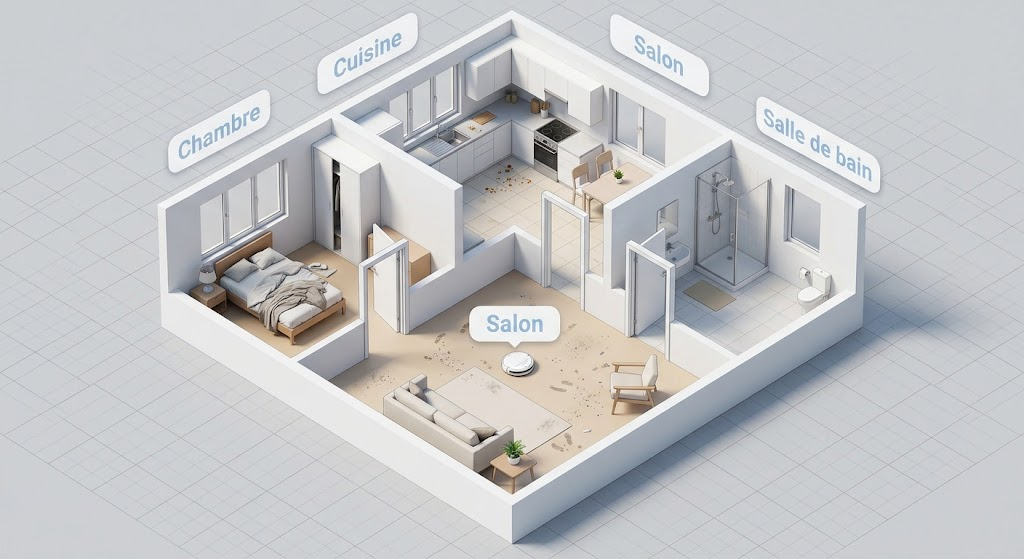
\includegraphics[width=0.7\textwidth]{captures/vue_3D_n.png}
		\caption{Topologie du logement. Le salon est le nœud central.}
		\label{fig:logement}
	\end{figure}
	
	Cette configuration en étoile est volontaire : elle rend le problème plus
	intéressant qu'un simple couloir, parce que le robot est obligé de revenir
	régulièrement au salon entre deux pièces. Elle oblige aussi à réfléchir à
	l'ordre dans lequel visiter les pièces pour éviter les allers-retours
	inutiles.
	
	\subsection{État initial et objectif}
	
	L'état initial est simple à décrire. Le robot se trouve dans le salon, et
	toutes les pièces sont sales, y compris le salon. Les passages entre les
	pièces sont tous disponibles.
	
	L'objectif est que toutes les pièces soient propres à la fin de l'exécution
	du plan. Nous ne demandons pas que le robot termine dans une pièce
	particulière, ni qu'il économise ses déplacements : seul compte le résultat
	final sur l'état des pièces.
	
	\subsection{Choix des prédicats}
	
	Pour décrire cette situation en PDDL, nous avons retenu quatre prédicats.
	
	Le prédicat \texttt{robot-at} associe le robot à une pièce. C'est lui qui
	permet de savoir où se trouve le robot à chaque étape du plan. Sans lui,
	aucune action de déplacement ni de nettoyage ne pourrait être déclenchée,
	puisque les deux actions dépendent de la position du robot.
	
	Les prédicats \texttt{dirty} et \texttt{clean} décrivent l'état de propreté
	d'une pièce. Nous aurions pu nous contenter d'un seul prédicat \texttt{clean}
	et considérer qu'une pièce non propre est sale, mais garder les deux rend le
	modèle plus lisible et permet d'écrire des préconditions et des effets
	symétriques. L'action de nettoyage ajoute \texttt{clean} et retire
	\texttt{dirty}, ce qui évite toute ambiguïté sur l'état d'une pièce.
	
	Le prédicat \texttt{connected} indique qu'il existe un passage entre deux
	pièces. Il porte sur une paire de pièces et non sur le robot, car les
	passages sont une propriété du logement, pas du robot.
	
	\subsection{Choix des actions}
	
	Deux actions suffisent pour modéliser le comportement du robot.
	
	L'action \texttt{move} permet au robot de passer d'une pièce à une pièce
	voisine. Elle prend trois paramètres : le robot, la pièce de départ et la
	pièce d'arrivée. Sa précondition exige que le robot soit effectivement dans
	la pièce de départ et qu'un passage existe entre les deux pièces. Ses effets
	ajoutent la nouvelle position du robot et retirent l'ancienne, car le robot
	ne peut pas être dans deux pièces à la fois.
	
	L'action \texttt{clean} permet au robot de nettoyer la pièce où il se trouve.
	Elle prend deux paramètres : le robot et la pièce. Sa précondition exige que
	le robot soit dans la pièce et que celle-ci soit sale. Ses effets ajoutent
	le fait que la pièce est propre et retirent le fait qu'elle est sale.
	
	Nous avons volontairement écarté d'autres actions, comme l'ouverture d'une
	porte ou l'utilisation d'un outil spécifique, pour garder le domaine aussi
	proche que possible des exemples classiques de planification STRIPS et pour
	que la difficulté principale reste l'ordonnancement des visites.
	
	\subsection{Difficulté rencontrée sur les passages}
	
	Un point nous a demandé un peu de réflexion : la direction des passages.
	Notre premier réflexe a été de déclarer un passage entre deux pièces une
	seule fois, par exemple \texttt{(connected salon cuisine)}. Le planificateur
	trouvait alors des plans pour aller de la cuisine vers le salon, mais pas
	l'inverse, alors que physiquement un passage se parcourt dans les deux sens.
	Nous avons donc ajouté systématiquement les deux faits, \texttt{(connected
		salon cuisine)} et \texttt{(connected cuisine salon)}, pour chaque liaison.
	C'est une contrainte du formalisme STRIPS, qui ne connaît pas la notion de
	relation symétrique : ce qui est vrai dans un sens doit être écrit
	explicitement dans l'autre.
	
	\section{Écriture en PDDL}
	
	\subsection{Domaine}
	
	Le domaine décrit les objets manipulés, les prédicats qui portent sur ces
	objets, et les actions que le robot peut exécuter. Il est indépendant du
	logement particulier : le même domaine pourrait servir pour un logement à
	cinq, six ou dix pièces.
	
	Nous définissons deux types d'objets, \texttt{robot} et \texttt{room}. Le
	typage permet au planificateur de vérifier que les paramètres passés aux
	actions sont cohérents et évite certaines erreurs d'écriture.
	
	\begin{lstlisting}[style=pddl, caption={Déclaration des types et des prédicats du domaine.}]
		(:types robot room)
		
		(:predicates
		(robot-at ?r - robot ?p - room)
		(dirty    ?p - room)
		(clean    ?p - room)
		(connected ?p1 - room ?p2 - room))
	\end{lstlisting}
	
	L'action de déplacement prend trois paramètres : le robot, la pièce de
	départ et la pièce d'arrivée. Sa précondition exige que le robot soit dans
	la pièce de départ et qu'il existe un passage entre les deux pièces. Son
	effet déplace le robot : il ajoute le fait \texttt{robot-at} sur la pièce
	d'arrivée et retire le fait \texttt{robot-at} sur la pièce de départ.
	
	\begin{lstlisting}[style=pddl, caption={Action de déplacement.}]
		(:action move
		:parameters (?r - robot ?from - room ?to - room)
		:precondition (and
		(robot-at ?r ?from)
		(connected ?from ?to))
		:effect (and
		(robot-at ?r ?to)
		(not (robot-at ?r ?from))))
	\end{lstlisting}
	
	L'action de nettoyage prend deux paramètres : le robot et la pièce à
	nettoyer. Sa précondition exige que le robot soit dans cette pièce et que
	la pièce soit sale. Son effet rend la pièce propre, en ajoutant
	\texttt{clean} et en retirant \texttt{dirty}.
	
	\begin{lstlisting}[style=pddl, caption={Action de nettoyage.}]
		(:action clean
		:parameters (?r - robot ?p - room)
		:precondition (and
		(robot-at ?r ?p)
		(dirty ?p))
		:effect (and
		(clean ?p)
		(not (dirty ?p))))
	\end{lstlisting}
	
	Le domaine est déclaré avec les prérequis \texttt{:strips} et
	\texttt{:typing}. Le premier indique qu'on se limite à la planification
	STRIPS classique, sans conditionnelles ni effets quantifiés. Le second
	autorise l'usage des types.
	
	\subsection{Problème}
	
	Le fichier de problème décrit une instance précise du domaine : les objets
	concrets, l'état initial et l'objectif.
	
	Les objets sont le robot \texttt{r1} et les quatre pièces
	\texttt{cuisine}, \texttt{salon}, \texttt{chambre} et \texttt{sdb}.
	
	\begin{lstlisting}[style=pddl, caption={Objets du problème.}]
		(:objects
		r1 - robot
		cuisine salon chambre sdb - room)
	\end{lstlisting}
	
	L'état initial place le robot dans le salon, déclare les quatre pièces
	sales, et précise les passages disponibles. Chaque passage est écrit dans
	les deux sens, comme nous l'avons expliqué dans la section précédente.
	
	\begin{lstlisting}[style=pddl, caption={État initial.}]
		(:init
		(robot-at r1 salon)
		(dirty cuisine) (dirty salon) (dirty chambre) (dirty sdb)
		(connected salon cuisine) (connected cuisine salon)
		(connected salon chambre) (connected chambre salon)
		(connected salon sdb)     (connected sdb salon))
	\end{lstlisting}
	
	L'objectif demande que les quatre pièces soient propres. Aucune contrainte
	n'est imposée sur la position finale du robot.
	
	\begin{lstlisting}[style=pddl, caption={Objectif.}]
		(:goal (and
		(clean cuisine)
		(clean salon)
		(clean chambre)
		(clean sdb)))
	\end{lstlisting}
	
	\subsection{Remarques sur la syntaxe}
	
	Deux points nous ont posé problème au moment de l'écriture.
	
	Le premier concerne le typage. Lorsqu'on écrit \texttt{?p - room}, il faut
	que \texttt{room} ait bien été déclaré dans la section \texttt{:types} du
	domaine. Une erreur de frappe sur un nom de type provoque un message du
	planificateur qui n'est pas toujours explicite, et il faut relire le
	fichier en entier pour trouver l'incohérence.
	
	Le second concerne les parenthèses. En PDDL, chaque prédicat est entouré de
	parenthèses, chaque action aussi, et l'ensemble de la définition est
	lui-même entre parenthèses. Une parenthèse manquante, même au niveau le
	plus externe, fait échouer l'analyse syntaxique. Nous avons pris l'habitude
	de compter les parenthèses ouvrantes et fermantes à chaque modification du
	fichier, et d'indenter systématiquement les blocs \texttt{:precondition} et
	\texttt{:effect} pour repérer visuellement les déséquilibres.
	
	\section{Utilisation de Fast Downward}
	
	\subsection{Installation}
	
	Fast Downward est un planificateur développé en C++ et distribué sous forme
	de code source. Son installation se fait en trois étapes : installer les
	dépendances, récupérer le dépôt, puis compiler le projet.
	
	Les dépendances nécessaires sont un compilateur C++, l'outil de
	construction CMake, l'outil \texttt{make} et Python 3. Sur une distribution
	Ubuntu, on les installe avec la commande suivante.
	
	\begin{lstlisting}[style=bash, caption={Installation des dépendances.}]
		sudo apt update
		sudo apt install -y cmake g++ make python3 git
	\end{lstlisting}
	
	On récupère ensuite le dépôt officiel de Fast Downward depuis GitHub, puis
	on se place dans le dossier ainsi créé.
	
	\begin{lstlisting}[style=bash, caption={Clone du dépôt Fast Downward.}]
		cd ~
		git clone https://github.com/aibasel/downward.git
		cd downward
	\end{lstlisting}
	
	La compilation se lance avec le script \texttt{build.py} fourni par le
	projet. Elle prend quelques minutes et produit un binaire dans le
	sous-dossier \texttt{builds/release/bin/}. On peut accélérer la compilation
	en indiquant le nombre de cœurs disponibles, par exemple avec l'option
	\texttt{-j4}.
	
	\begin{lstlisting}[style=bash, caption={Compilation de Fast Downward.}]
		./build.py -j4
	\end{lstlisting}
	
	Une fois la compilation terminée, le message
	\texttt{Built configuration release successfully.} confirme que tout s'est
	bien passé. On peut vérifier la version installée avec l'option
	\texttt{--version}.
	
	\begin{lstlisting}[style=bash, caption={Vérification de l'installation.}]
		./fast-downward.py --version
	\end{lstlisting}
	
	\subsection{Lancement du planificateur}
	
	Fast Downward s'utilise en lui passant un fichier de domaine, un fichier de
	problème et une méthode de recherche. Le script
	\texttt{fast-downward.py} sert de point d'entrée : il appelle d'abord le
	traducteur, qui convertit les fichiers PDDL en une représentation interne,
	puis il lance la recherche à proprement parler.
	
	\begin{lstlisting}[style=bash, caption={Lancement sur le scénario 1.}]
		python3 ~/downward/fast-downward.py \
		domain.pddl problem.pddl \
		--search "astar(blind())"
	\end{lstlisting}
	
	Le plan produit est écrit dans un fichier \texttt{sas\_plan} à côté du
	répertoire courant. On peut aussi le rediriger vers un fichier choisi, par
	exemple \texttt{plan.txt}, en ajoutant une redirection à la fin de la
	commande.
	
	\subsection{Choix de la méthode de recherche}
	
	Fast Downward propose plusieurs algorithmes de recherche. Nous avons retenu
	\texttt{astar(blind())}, qui combine la recherche A* avec une heuristique
	dite aveugle. L'heuristique aveugle renvoie toujours zéro : elle
	n'apporte aucune information sur la distance au but, mais elle garantit que
	la recherche reste optimale en nombre d'actions.
	
	Ce choix est adapté à notre problème pour deux raisons. D'abord, l'espace
	d'états est très petit : quatre pièces, quatre objets de propreté, et une
	position de robot, ce qui donne un nombre d'états explorables rapidement.
	Ensuite, comme l'heuristique aveugle ne peut pas se tromper, le plan trouvé
	est nécessairement de coût minimal. Nous avons donc l'assurance que les
	neuf actions du scénario 1 sont le strict minimum pour atteindre le but.
	
	Sur un problème plus grand, on préférerait sans doute une heuristique plus
	informative, comme \texttt{hmax} ou \texttt{lmcut}, pour éviter que la
	recherche n'explore inutilement de nombreux états. Ici, ce n'était pas
	nécessaire.
	
	\subsection{Lecture du plan}
	
	Sur le scénario 1, le planificateur trouve une solution en quelques
	millisecondes. Le plan comporte neuf actions.
	
	\begin{lstlisting}[style=pddl, caption={Plan produit pour le scénario 1.}]
		move  r1 salon chambre
		clean r1 chambre
		move  r1 chambre salon
		move  r1 salon cuisine
		clean r1 cuisine
		move  r1 cuisine salon
		clean r1 salon
		move  r1 salon sdb
		clean r1 sdb
	\end{lstlisting}
	
	La lecture de ce plan confirme la structure du logement. Le robot commence
	par aller dans la chambre, la nettoie, revient au salon, va dans la cuisine,
	la nettoie, revient au salon et profite de ce passage pour nettoyer le
	salon, puis se rend dans la salle de bain et la nettoie. Chaque aller vers
	une pièce périphérique est suivi d'un retour au salon, ce qui est la
	conséquence directe de la topologie en étoile : le salon est le seul point
	de passage entre les trois autres pièces.
	
	Le salon est nettoyé à l'étape sept, après le retour depuis la cuisine.
	Cet ordre n'est pas unique : le planificateur aurait pu nettoyer le salon
	dès le début, à l'étape zéro, et le résultat aurait été le même en nombre
	d'actions. Avec une heuristique aveugle, l'ordre exact dépend de l'ordre
	d'exploration des successeurs, mais la longueur du plan reste optimale.
	
	\section{Vérification et scénarios alternatifs}
	
	\subsection{Simulateur Python}
	
	Fast Downward produit un plan, mais rien ne garantit qu'il soit exécutable
	dans les termes du problème. Nous avons écrit un simulateur Python
	indépendant pour rejouer le plan action par action et vérifier les
	préconditions.
	
	L'état est représenté par un dictionnaire : position du robot, ensemble des
	pièces sales, ensemble des pièces propres. La fonction qui applique une
	action vérifie les préconditions par des assertions.
	
	\begin{lstlisting}[style=python, caption={Application d'une action.}]
		def apply(state, action):
		if action[0] == "move":
		_, src, dst = action
		assert state["robot"] == src
		assert (src, dst) in CONNECTIONS
		state["robot"] = dst
		elif action[0] == "clean":
		_, room = action
		assert state["robot"] == room
		assert room in state["dirty"]
		state["dirty"].remove(room)
		state["clean"].add(room)
	\end{lstlisting}
	
	Sur le scénario 1, la simulation se termine sans erreur et confirme que les
	quatre pièces sont propres. Elle montre aussi que le salon est nettoyé
	après le retour depuis la cuisine, alors qu'il aurait pu l'être dès la
	première action : le plan est optimal en longueur, mais pas unique.
	
	\subsection{Scénario 2 : cuisine déjà propre}
	
	La cuisine est déclarée propre dans l'état initial ; le but reste
	inchangé. Le planificateur retourne un plan de six actions.
	
	\begin{lstlisting}[style=pddl, caption={Plan du scénario 2.}]
		move  r1 salon chambre
		clean r1 chambre
		move  r1 chambre salon
		clean r1 salon
		move  r1 salon sdb
		clean r1 sdb
	\end{lstlisting}
	
	Le robot ne visite plus la cuisine. L'action \texttt{clean} exige en
	précondition que la pièce soit sale ; comme la cuisine est déjà propre,
	cette action n'est jamais applicable, et le plan économise trois étapes
	par rapport au scénario 1. Ce résultat montre que les préconditions
	orientent la recherche en éliminant les branches inutiles.
	
	\subsection{Scénario 3 : salle de bain inaccessible}
	
	Le passage entre le salon et la salle de bain est retiré ; les autres
	conditions sont identiques au scénario 1. Fast Downward ne trouve aucun
	plan et affiche :
	
	\begin{lstlisting}[style=base, caption={Sortie de Fast Downward.}]
		No relaxed solution! Generating unsolvable task...
		Initial state is a dead end.
		Search terminated -- no plan exists!
		Task is provably unsolvable.
	\end{lstlisting}
	
	Sans passage vers la salle de bain, aucune action \texttt{move} ne peut y
	conduire le robot, donc le fait \texttt{(clean sdb)} demandé dans le but
	est impossible à produire. Le traducteur détecte cette impossibilité avant
	même la recherche.
	
	\subsection{Comparaison}
	
	\begin{table}[h]
		\centering
		\begin{tabular}{l l l l}
			\hline
			Scénario & Modification & Résultat & Plan \\
			\hline
			1 & aucune & solution & 9 actions \\
			2 & cuisine propre & solution & 6 actions \\
			3 & passage retiré & insoluble & -- \\
			\hline
		\end{tabular}
		\caption{Comparaison des trois scénarios.}
	\end{table}
	
	Les deux variantes confirment le comportement attendu du modèle. Le
	scénario 2 montre qu'une précondition non satisfaite élimine une branche
	inutile et raccourcit le plan. Le scénario 3 montre qu'une seule connexion
	en moins suffit à rendre le but inatteignable, ce que le planificateur
	signale sans produire de plan incorrect.
	
	\section{Difficultés rencontrées}
	
	Deux points nous ont ralenti pendant la mise en place, sans remettre en
	cause la démarche.
	
	La compilation de Fast Downward a été interrompue une première fois, par
	impatience, alors qu'elle durait depuis plusieurs minutes. Le message
	\texttt{KeyboardInterrupt} affiché dans le terminal n'était pas une erreur
	du planificateur mais la conséquence directe de cette interruption
	manuelle. Nous avons relancé la compilation en la laissant aller au bout,
	et elle s'est terminée normalement.
	
	Du côté de l'écriture PDDL, plusieurs erreurs de syntaxe nous ont coûté du
	temps. Une parenthèse manquante au niveau d'un bloc \texttt{:effect} suffit
	à faire échouer l'analyse du fichier, et le message renvoyé par le
	planificateur ne pointe pas toujours la ligne exacte. Nous avons pris
	l'habitude d'indenter systématiquement les préconditions et les effets, et
	de vérifier l'équilibre des parenthèses après chaque modification. La même
	précaution s'applique aux noms de types : une faute de frappe sur
	\texttt{room} ou \texttt{robot} provoque une erreur d'instanciation qui
	n'est pas toujours facile à localiser.
	
	\section{Conclusion}
	
	Ce TP nous a fait parcourir l'ensemble de la chaîne de planification
	classique, depuis la description informelle d'un problème jusqu'à la
	vérification d'un plan exécutable. Le passage de la description en langage
	naturel à un modèle STRIPS nous a obligés à identifier précisément ce qui
	constitue un état, ce qui distingue une précondition d'un effet, et ce que
	signifie atteindre un but. Nous avons également constaté qu'un plan
	optimal en longueur n'est pas nécessairement unique, et que le rôle du
	planificateur se limite à trouver une séquence d'actions cohérente avec le
	modèle qu'on lui a fourni.
	
	Le modèle que nous avons écrit couvre la topologie du logement et l'état de
	propreté des pièces, mais il laisse de côté plusieurs aspects du problème
	réel. Le robot ne dispose pas de batterie, ne met pas de temps à se
	déplacer, ne rencontre pas d'obstacles et ne peut pas échouer dans son
	nettoyage. Chacune de ces dimensions pourrait être ajoutée, mais elle
	nécessiterait des prédicats supplémentaires et rendrait la recherche plus
	coûteuse : la simplicité du modèle actuel est aussi ce qui permet au
	planificateur de trouver une solution en quelques millisecondes.
	
	Plusieurs pistes d'amélioration seraient envisageables. On pourrait
	introduire une notion de coût différencié entre les déplacements et les
	nettoyages, pour que le planificateur privilégie les plans qui minimisent
	le temps plutôt que le nombre d'actions. On pourrait également ajouter des
	pièces supplémentaires ou des passages multiples entre deux pièces, afin
	d'étudier comment le plan évolue quand le graphe devient plus riche.
	Enfin, on pourrait comparer plusieurs heuristiques de Fast Downward sur le
	même problème pour observer l'effet du choix de la méthode de recherche
	sur le temps de calcul et sur la qualité du plan produit.
	
	% ============================================================
	% ANNEXES
	% ============================================================
	\appendix
	\renewcommand{\thesection}{\Alph{section}}
	
	
	\newpage
	\section{Fichier \texttt{domain.pddl}}
	
	\begin{lstlisting}[style=pddl, caption={Domaine complet.}]
		(define (domain aspirateur)
		(:requirements :strips :typing)
		(:types robot room)
		
		(:predicates
		(robot-at ?r - robot ?p - room)
		(dirty ?p - room)
		(clean ?p - room)
		(connected ?p1 - room ?p2 - room))
		
		(:action move
		:parameters (?r - robot ?from - room ?to - room)
		:precondition (and
		(robot-at ?r ?from)
		(connected ?from ?to))
		:effect (and
		(robot-at ?r ?to)
		(not (robot-at ?r ?from))))
		
		(:action clean
		:parameters (?r - robot ?p - room)
		:precondition (and
		(robot-at ?r ?p)
		(dirty ?p))
		:effect (and
		(clean ?p)
		(not (dirty ?p)))))
	\end{lstlisting}
	
	\section{Fichier \texttt{problem.pddl} (scénario 1)}
	
	\begin{lstlisting}[style=pddl, caption={Problème du scénario 1.}]
		(define (problem aspirateur-1)
		(:domain aspirateur)
		(:objects
		r1 - robot
		cuisine salon chambre sdb - room)
		(:init
		(robot-at r1 salon)
		(dirty cuisine) (dirty salon) (dirty chambre) (dirty sdb)
		(connected salon cuisine) (connected cuisine salon)
		(connected salon chambre) (connected chambre salon)
		(connected salon sdb)     (connected sdb salon))
		(:goal (and
		(clean cuisine)
		(clean salon)
		(clean chambre)
		(clean sdb))))
	\end{lstlisting}
	
	\section{Simulateur Python}
	
	\begin{lstlisting}[style=python, caption={Simulateur complet.}]
		ROOMS = ["cuisine", "salon", "chambre", "sdb"]
		
		CONNECTIONS = {
			("salon", "cuisine"), ("cuisine", "salon"),
			("salon", "chambre"), ("chambre", "salon"),
			("salon", "sdb"),     ("sdb", "salon"),
		}
		
		state = {
			"robot": "salon",
			"dirty": {"cuisine", "salon", "chambre", "sdb"},
			"clean": set(),
		}
		
		plan = [
		("move",  "salon", "chambre"),
		("clean", "chambre"),
		("move",  "chambre", "salon"),
		("move",  "salon", "cuisine"),
		("clean", "cuisine"),
		("move",  "cuisine", "salon"),
		("clean", "salon"),
		("move",  "salon", "sdb"),
		("clean", "sdb"),
		]
		
		def apply(state, action):
		if action[0] == "move":
		_, src, dst = action
		assert state["robot"] == src
		assert (src, dst) in CONNECTIONS
		state["robot"] = dst
		elif action[0] == "clean":
		_, room = action
		assert state["robot"] == room
		assert room in state["dirty"]
		state["dirty"].remove(room)
		state["clean"].add(room)
		
		for act in plan:
		apply(state, act)
		
		assert state["clean"] == set(ROOMS)
		print("PLAN VALIDE : toutes les pieces sont propres.")
	\end{lstlisting}
	
	\section{Captures}
	
	
	
	\begin{figure}[h]
		\centering
		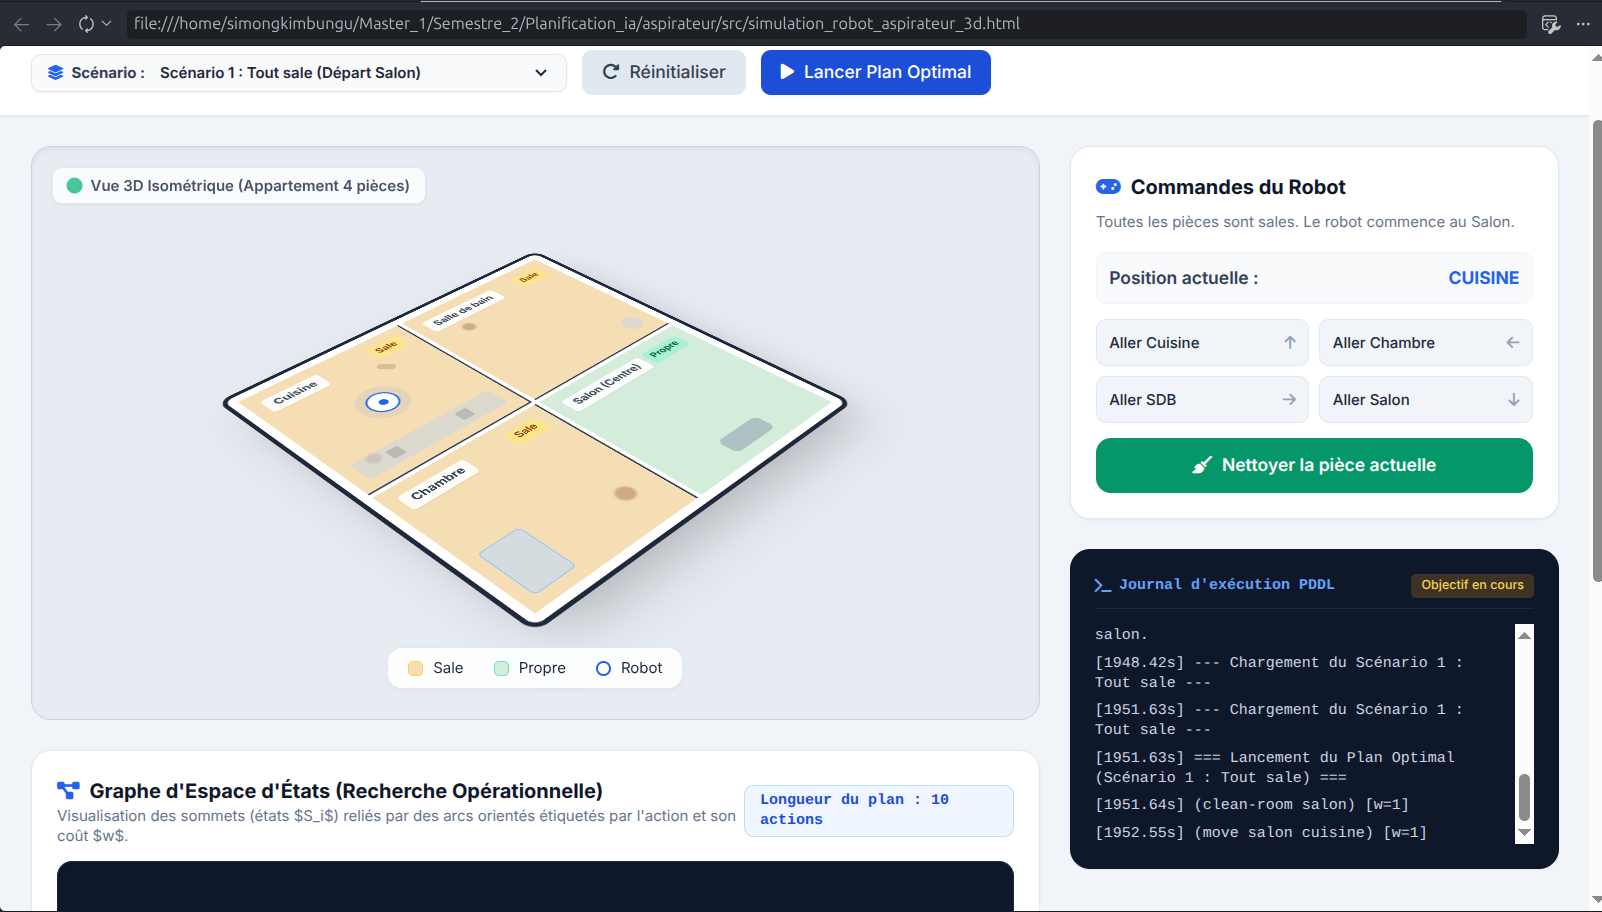
\includegraphics[width=0.85\textwidth]{captures/simulateur_3d.png}
		\caption{Sortie du simulateur Python.}
	\end{figure}
	
\end{document}